\section{Event generation}
\label{chp:evtsim:evtgen}

The modelling of a $pp$ collision requires a detailed understanding of the dynamics of a deep-inelastic interaction at high energy (perturbative QCD), as well as the structure of a relativistic proton and the evolution of partons into stable hadrons at very low energy (non-perturbative QCD). The complication of collisions involving protons is that protons are composite particles, thus a precise understanding of the partonic structure of the proton is needed to calculate the process cross section. A proton is a bound state composed of point-like quarks and gluons interacting among themselves via the constant exchange of soft virtual gluons. According to the uncertainty principle, the time scale of a virtual gluon interaction is inversely proportional to its virtuality $q$, i.e. t $\sim1/q$, so that gluons with higher virtuality usually are absorbed by the same quark by which they were radiated. A hard probe interacts within a much shorter timescale $1/Q \ll 1/q$ during which the partonic fluctuations in the struck proton appear almost frozen. The hard probe effectively takes a snapshot of the proton structure, at a characteristic resolution given by $\sim1/Q$. The independence of long-wavelength (soft) structure on the nature of the hard (short-distance) process, a key aspect in the simulation of $pp$ collision, gives the possibility of factorizing the different processes happening at different energy scales (factorisation theorem).
Since the interaction cross section of such collisions decreases as the momentum exchange $Q$ between the colliding particles increases, a $pp$ collision typically consists of one so-called hard scattering/process with a high momentum exchange $Q$ computed at a fixed order (e.g. next-to-leading order, NLO) in perturbation theory, which is sometimes accompanied by further soft collisions, so-called multi-parton interactions that are instead described via phenomenological models.

\bfig[h!]
\centering
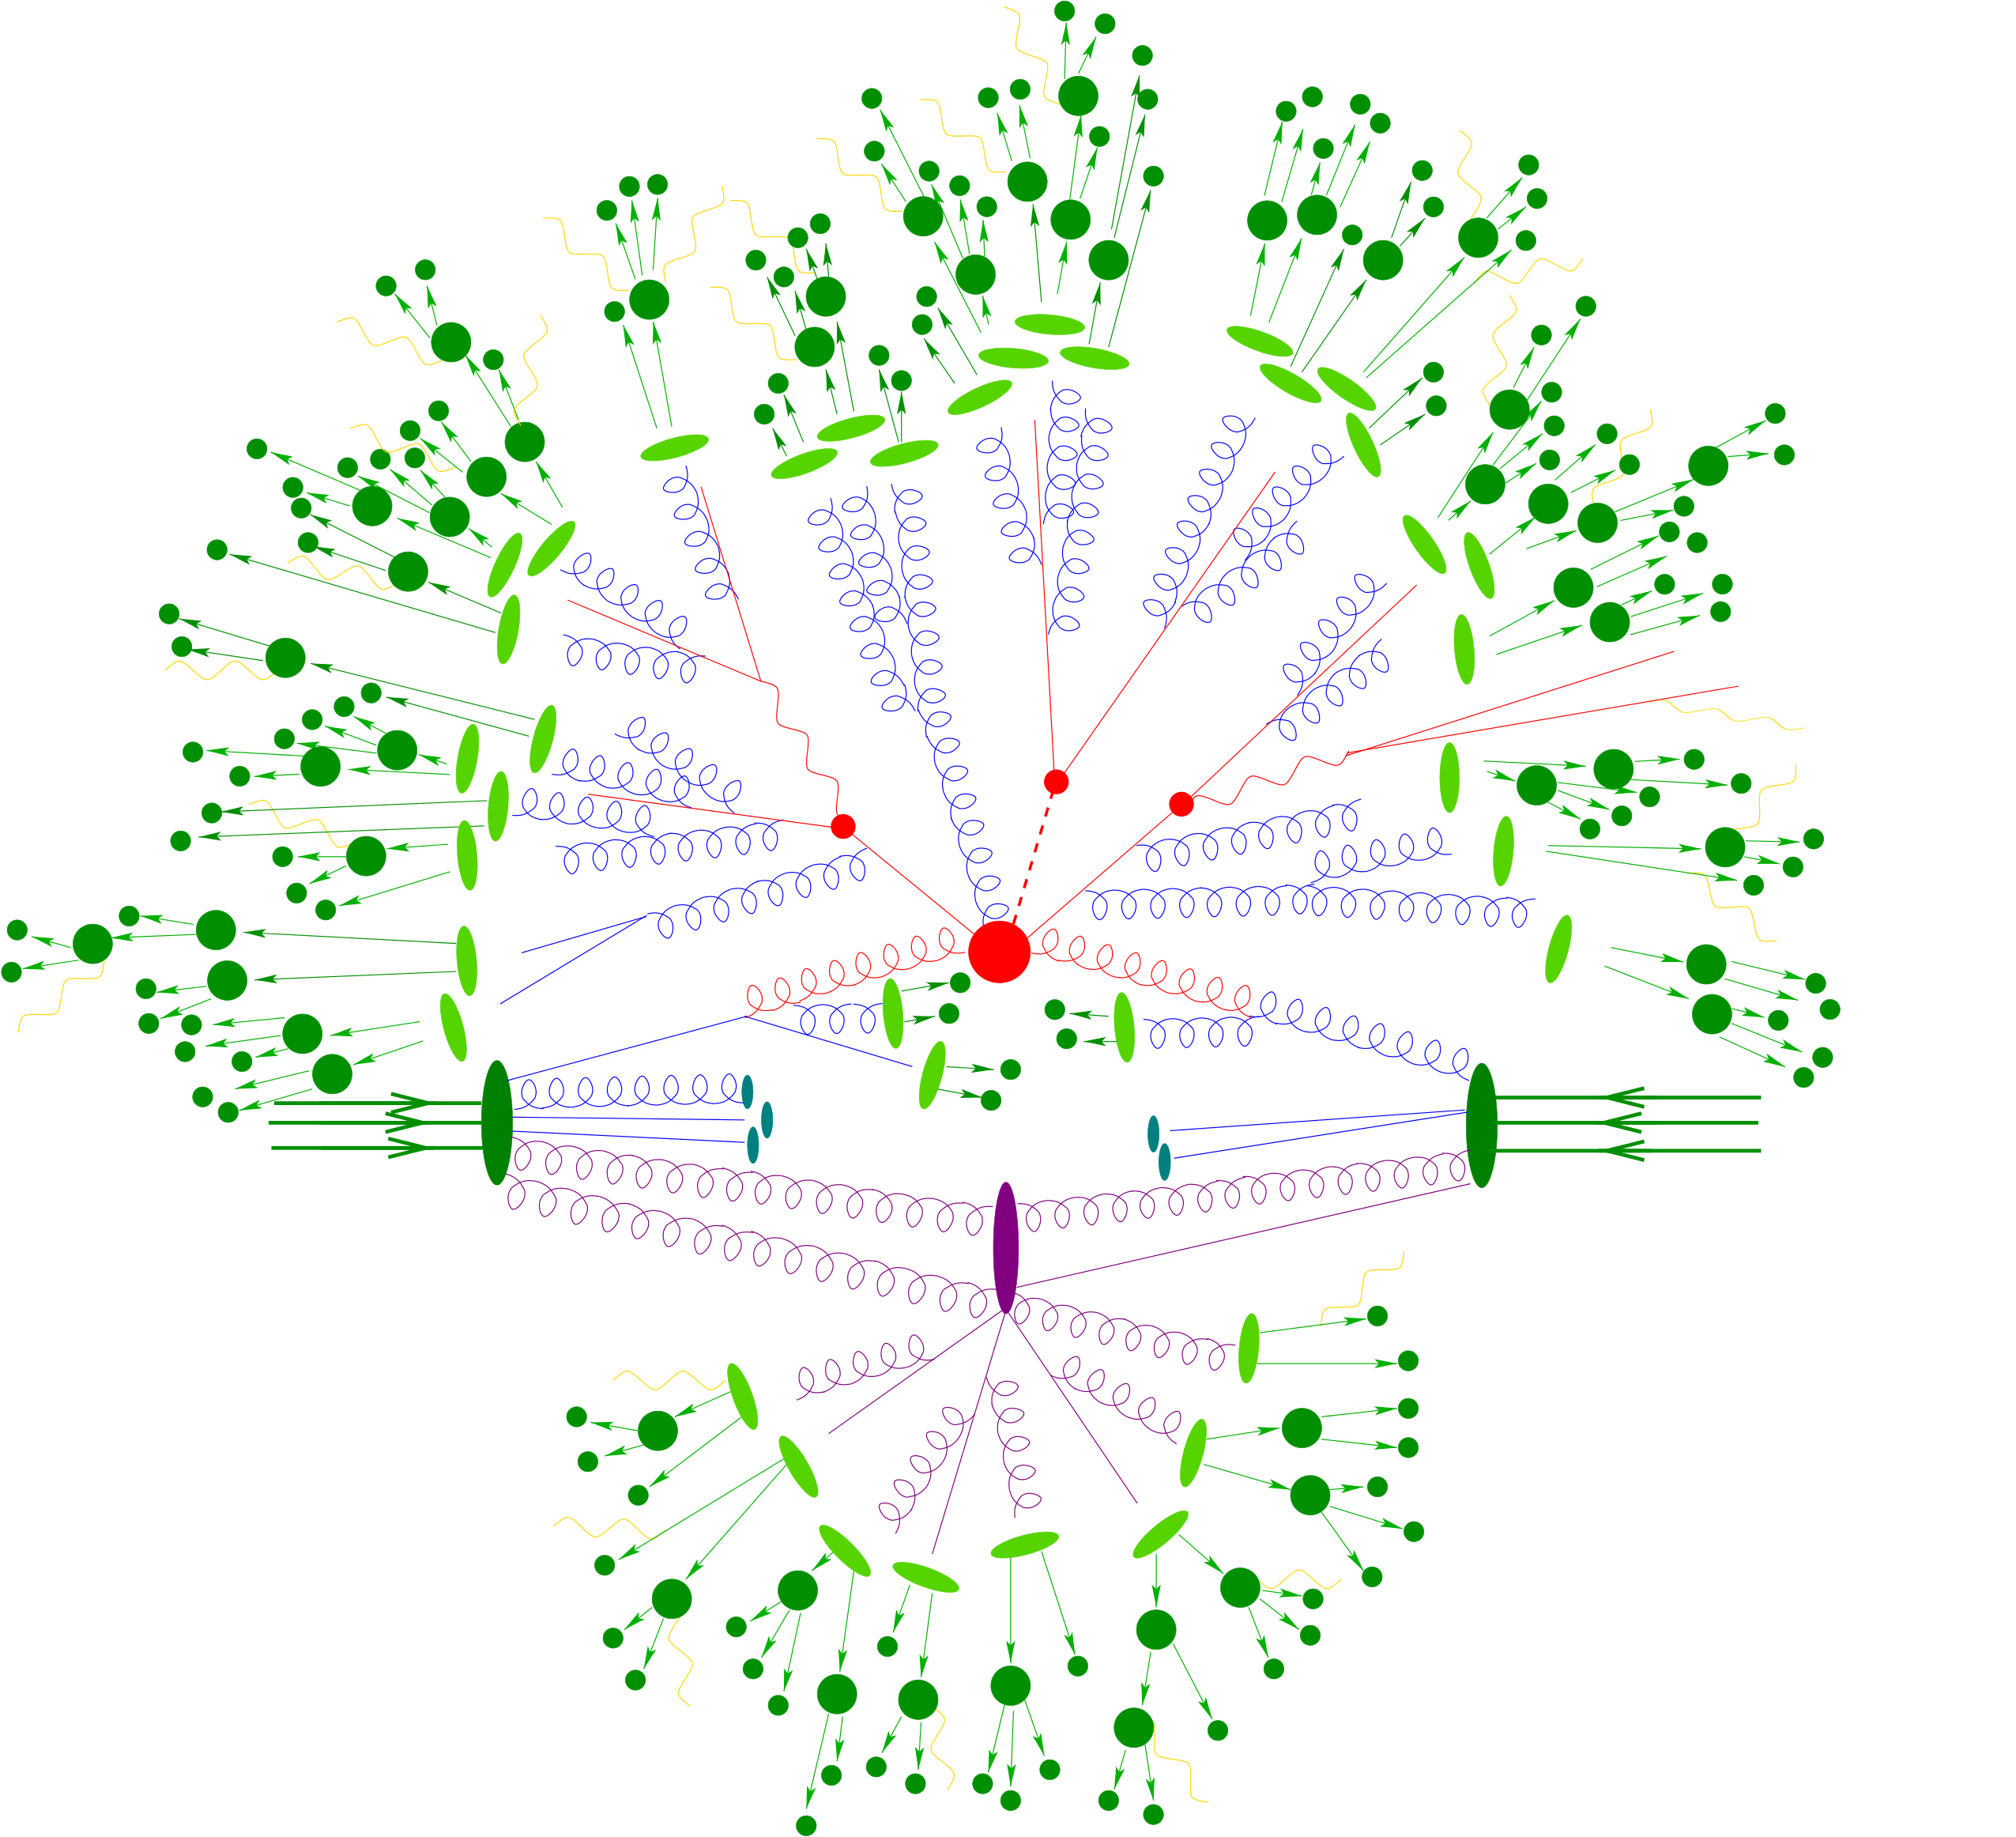
\includegraphics[width=0.8\textwidth]{figures/EvtGen/event}
\captionsetup{width=0.85\textwidth} \caption{\small Illustration of a $pp$ collision. Two partons from the incoming protons (large green ellipses) undergo initial state radiation and interact in the hard process (big red blob). A parton shower (red) emerges from the products of the hard interaction. The resulting partons hadronise into colourless states (light green blobs) that subsequently decay into stable particles (green circles). A secondary interaction between proton remnants is shown as a purple blob, again creating a parton shower (purple), which hadronises, followed by decays into stable particles. This is part of the underlying event, together with the beam remnants (light blue blobs). Electromagnetic radiation (yellow) can be emitted by charged particles at any stage. From reference \cite{Siegert:2010cru}.}
\label{sec:evtgen:fig:evt}
\efig

\subsection{Factorisation theorem}
\label{chp:evtsim:evtgen:hp}

The event simulation begins with the collision, with large momentum transfer, between two partons within the protons. At high energy, the partons behave as asymptotically free, and a perturbative description is applied. The cross section for a generic process $pp \to X$ is defined in terms of the cross section for the partonic processes, according to the factorisation theorem \cite{Collins:1989gx}, as

\be
\sigma_{pp \to X}= \displaystyle\sum_{a,b} \int dx_{a}dx_{b} f_{a}(x_{a},\mu_{F}^{2}) f_{b}(x_{b},\mu_{F}^{2}) \hat{\sigma}_{ab\to X}(x_{a}p_{a},x_{b}p_{b},\mu_{R}^{2},\mu_{F}^{2}),
\ee

\noindent where the sum runs over all possible combinations of the partons $a$ and $b$ able to produce $X$. The parton density function (PDF), $f_{i}(x_{i},\mu_{F}^{2})$, represents the effective density of partons of type/flavor $i$, as a function of the momentum fraction $x_{i}$, when a hadron is probed at a scale $\mu_{F}$. The factorisation scale $\mu_{F}$ represents the estimated limit between the perturbative and non-perturbative QCD regimes, i.e. the energy at which the running $\alpha_{s}$ becomes too large for achieving a desired convergence of the perturbation series. In addition, the cross section calculation depends on the choice of the renormalisation scale $\mu_{R}$ of QCD, at which $\alpha_{s}$ is evaluated. As the factorisation and renormalisation scales describe the not precisely known boundaries between two physics domains, their values are usually related to some quantities characteristic of the modelled process (e.g. the mass of the particle produced, or the sum of the momenta of outgoing particles). The uncertainties arising from such a convention are typically estimated by comparing the cross section values $\sigma_{pp\to X}$ evaluated varying the nominal scale choice for $\mu_{F}$ or $\mu_{R}$ by a factor of two up and down. The cross section for the partonic process $\hat{\sigma}_{ab\to X}(x_{a}p_{a},x_{b}p_{b},\mu_{R}^{2},\mu_{F}^{2})$  is computed explicitly at a fixed order in perturbation theory. This step is also referred to as Matrix Element (ME) calculation, because it involves the calculation of the scattering matrix relating the initial and final state particles of the process.

\bfig[h!]
\centering
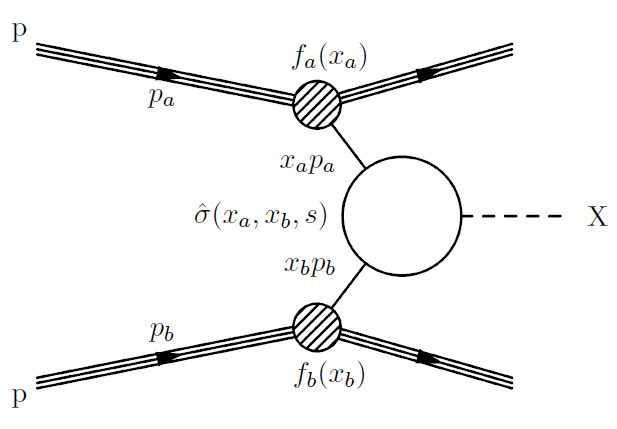
\includegraphics[width=0.6\textwidth]{figures/EvtGen/hs.png}
\captionsetup{width=0.85\textwidth} \caption{\small Illustration of a hard scattering. A parton with four-momentum $x_{a}p_{a}$, originating from a proton with a four-momentum $p_{a}$, undergoes a hard collision with a parton carrying a four-momentum  $x_{b}p_{b}$, coming from a proton with a four-momentum $p_{b}$. The spectator partons do not influence the hard interaction and continue their trajectory with slightly distorted directions.
}
\label{sec:evtgen:fig:hs}
\efig


\subsection{Parton density functions}
\label{chp:evtsim:evtgen:pdf}
QCD does not predict the structure of the proton and therefore the PDFs cannot be calculated, but have to be measured from experimental data. Historically, most of the information came from Deep-Inelastic Scattering (DIS) in fixed-target lepton-nucleon scattering experiments and from the HERA electron-proton collider at DESY. The energy dependence of the PDFs is given by the DGLAP evolution equations \cite{DGLAP1,DGLAP2,DGLAP3}:


\begin{equation}
\frac{\partial q_{i}(x,Q^{2})}{\partial \log Q^{2}}=\frac{\alpha_{s}}{2\pi} \int_x^1 \frac{dz}{z} \left \{ P_{q_{i}q_{j}}(z,\alpha_{s})q_{j}(\frac{x}{z},Q^{2}) + P_{q_{i}g}(z,\alpha_{s})g(\frac{x}{z},Q^{2})\right\},
\end{equation}
\begin{equation}
\frac{\partial g(x,Q^{2})}{\partial \log Q^{2}}=\frac{\alpha_{s}}{2\pi} \int_x^1 \frac{dz}{z} \left \{ P_{gq_{j}}(z,\alpha_{s})q_{j}(\frac{x}{z},Q^{2}) + P_{gg}(z,\alpha_{s})g(\frac{x}{z},Q^{2})\right\}.
\end{equation}

In the above expressions, $g(x,Q^{2})$ is the gluon PDF, $q_{i}(x,Q2)$ is the quark PDF, and $P_{ab}(z, Q^{2})$ are the splitting functions. 
For the evolution in $x$, there are no such equations, but it has to be obtained from fits to experimental data. Several collaborations continuously work to improve the PDF fits with the most recent data. PDF sets  from the groups CTEQ \cite{ct10}, NNPDF \cite{Ball:2012cx} and MSTW \cite{mstw1} are extensively used at the LHC.

\bfig[h!]
\centering
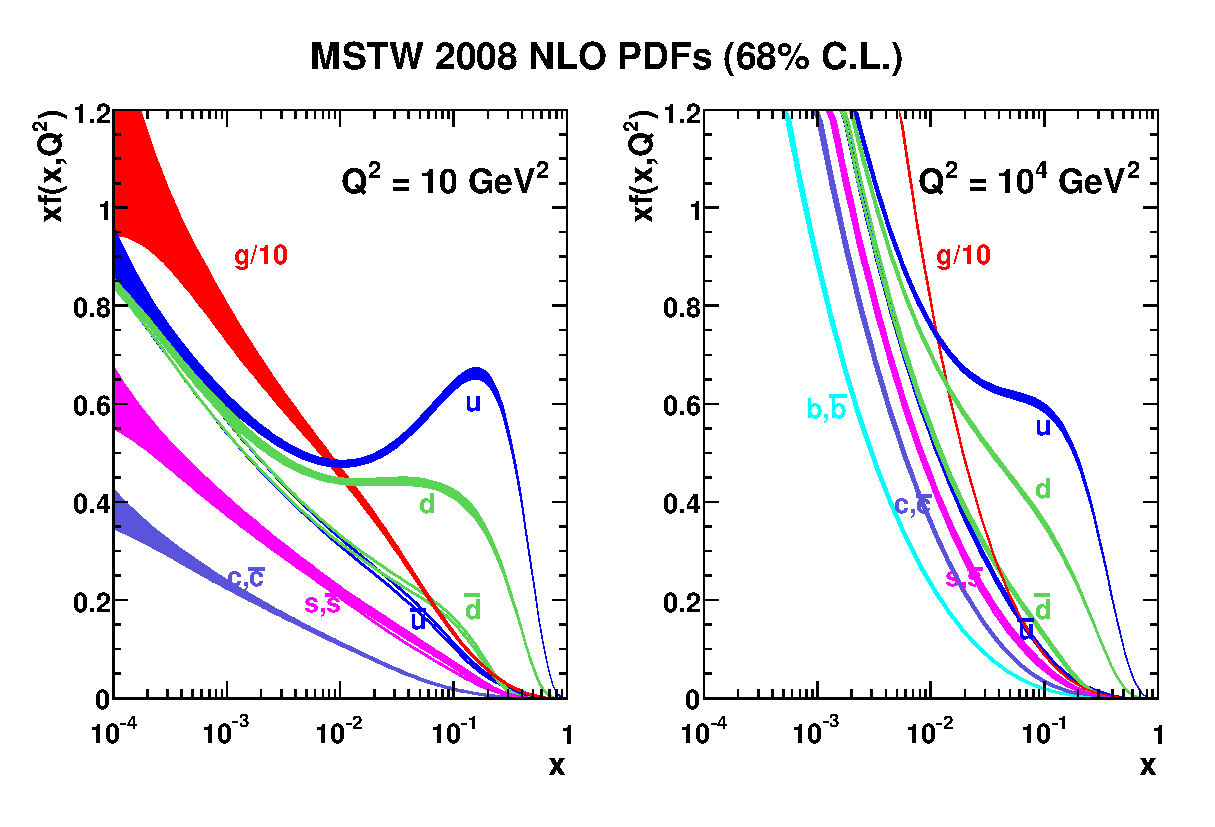
\includegraphics[width=0.7\textwidth]{figures/EvtGen/PDFplot.eps}
\captionsetup{width=0.85\textwidth} \caption{\small Parton luminosities for MSTW 2008 NLO PDF set as function of $x$ with the uncertainty band. On the left (right) panel for $Q^{2}=10$ $(10^{4})$ $\gev^{2}$. From reference \cite{mstw1}.}
\label{sec:evtgen:fig:pdf}
\efig


\subsection{Matrix element}

The production of an arbitrary final state, $ab \to X$, from a hadron collision can be expressed to all-orders in perturbation theory as:

\be
\hat{\sigma}_{ab\to X}= \underbrace{\displaystyle\sum_{k=0}^{\infty}\int d\Phi_{X+k}}_{\sum \rm legs}\underbrace{|\displaystyle\sum_{\ell=0}^{\infty}\mathcal{M}_{X+k}^{(\ell)}|^{2}}_{\sum \rm loops},
\ee

\noindent where $\mathcal{M}_{X+k}^{(\ell)}$ is the amplitude for producing $X$ in association with $k$ additional final-state partons (real emission corrections, or ``legs'')  and with $\ell$ additional virtual correction loops. The phase space of the configuration with $k$ legs is represented by $d\Phi_{X+k}$.  Specific values of $k+\ell$ will return the fixed-order calculations of perturbative QCD:
\bi
\ib $k=0$, $\ell=0$ $\implies$ LO (usually tree-level) for $X$ production;
\ib $k=n$, $\ell=0$ $\implies$ LO for $X$+$n$ jets;
\ib $k+\ell$ $\le$ n $\implies$ $N^{n}$LO for $X$ (includes $N^{n-1}$LO for $X$+1 jet, $N^{n-2}$LO for $X$+2 jets, and so on up to LO for $X+n$ jets ).
\ei


According to the KLN theorem \cite{KLN1,KLN2}, the infrared (IR) singularities coming from integrating over collinear and soft real-emission configurations should cancel, order by order, with those coming from the IR-divergent loop integrals.
However, in a fixed-order calculation, e.g. leading order, in the situation for which $k\ge1$, $\ell=0$, the integration over the full momentum phase space will include configurations in which one or more of the $k$ partons become collinear or soft. Such configurations leads to IR singularities in the integration region, which must be regulated cutting away the problematic regions of the phase space. The remaining part of the phase space is then considered by parton-shower generators.


\subsection{Parton shower}

Partons involved in a hard-scatter process normally have a very high energy ($Q>1$ $\gev$) for which $\alpha_{s}$ is small ($\ll$1). At such energies, quarks and gluons are likely to radiate off a gluon, carrying a portion of the energy of its mother particle and a colour connection to it. These gluons can then decay into further gluons or quark-antiquark pairs, leading to the formation of parton showers. This process continues as long as the particles produced have sufficient energy ($Q>1$ $\gev$) to reach a distance from the initial particle at which the colour field breaks up into a quark-antiquark pair.
Parton Showers (PS) populate regions of the phase space where emissions are collinear or soft (IR divergent) providing an all-orders resummation using an approximation scheme with a leading-logarithmic (``leading-log'') accuracy. The parton shower contribution to the hard process cross section is thus estimated by including only the dominant contribution to each order.
Starting from a differential cross section for $n$ particles $d\sigma_{n}$, a differential cross section for $n+1$ particles is calculated parametrising the probability that the new particle $j$ carries a fraction $z$ of the energy of its mother particle $i$ emitted at a virtuality scale or invariant mass $q^2$ using the splitting function $P_{ij}(z,q^{2})$:

\be
d\sigma_{n+1}\approx d\sigma_{n}\frac{\alpha_{s}}{2\pi}\frac{dq^{2}}{q^{2}}dz P_{ij}(z,q^{2}).
\label{eq:evtsim:evtgen:nplusone}
\ee

The simulation algorithm develops the shower by applying equation \ref{eq:evtsim:evtgen:nplusone} iteratively, for each parton involved in the hard interaction. The splitting functions obviously play a crucial role driving the emission probabilities. In MC simulations the formulation of parton shower uses a more convenient expression using the so-called Sudakov form factors:

\be
\Delta_{i}(q_{1}^{2},q_{2}^{2})=\exp\left( - \displaystyle\sum_{j \in q,g } \int_{q_{2}^{2}}^{q_{1}^{2}} \frac{dq^{2}}{q^{2}} \int_{z_{\rm min}}^{z_{\rm max}} \frac{\alpha_{s}}{4\pi} dz P_{ij}(z,q^{2})\right),
\label{eq:evtsim:evtgen:sudakov}
\ee

\noindent which represent the unconditional survival probability for a parton not to undergo a resolvable emission process between the two energy scales $q_{1}^{2}$ and $q_{2}^{2}$. The algorithm implemented in MC simulations goes through the following steps:
\bi
\ib Given the initial scale $Q^2$, referred to as resummation scale, it produces an emission at scale $q_{2}^{2}$ using equation \ref {eq:evtsim:evtgen:sudakov}.
\ib If the value of $q_{2}^{2}$ is lower than the hadronisation scale, $q_{2}^{2} \ll Q_{0}^{2} \approx 1$ $\gev^{2}$ no further emission occurs, thus the shower developments stops and hadronisation takes place.
\ib Otherwise, further emissions will occur and the process is repeated for each new parton using $q_{2}^{2}$ as initial scale.
\ei


Final-state radiation (FSR), i.e. a gluon radiated off a final-state parton is generated through the above parton shower procedure. For the initial-state radiation (ISR), however, this procedure is not suitable, as the momenta of the partons initiating the hard process need to be precisely adjusted to produce the hard process (e.g. a gluon decaying into a $t\bar{t}$ pair). Thus, the longitudinal momentum fractions $x_{1}$ and $x_{2}$ of the incoming partons need to be simulated first, and the momentum and angle of the ISR is found by backwards evolution, which involves a PDF-dependent correction to the Sudakov form factors. Due to the existing colour connections, the direction of the ISR tends to be aligned with that of mother parton.

\subsection{Matrix element and parton shower matching}

To improve the leading-log (LL) description given by the parton shower, it is often necessary to go beyond the approximations made in that step. One possibility is to replace the parton-shower approximation at given orders in the strong coupling expansion by exact perturbative QCD results. The left panel of the figure \ref{sec:evtgen:fig:dc} describes the LO cross section computation for some process $X$ and interfacing the parton shower to it.
\bfig[t!]
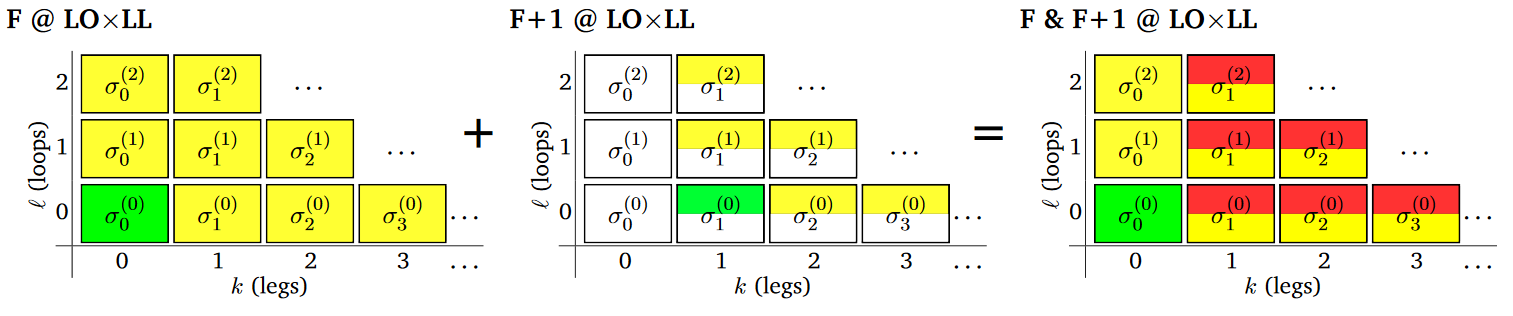
\includegraphics[width=\textwidth]{figures/EvtGen/doublecounting.png}
\captionsetup{width=0.85\textwidth} \caption{\small The double-counting problem caused by adding cross sections involving matrix elements with different numbers of legs when interfaced to parton showers. From reference \cite{Skands:2012ts}.}
\label{sec:evtgen:fig:dc}
\efig
This only gives a LL description of $X+1$ parton. To improve this precision LO matrix element for $X+1$ parton is added with an infrared cut-off to prevent divergences from soft and collinear emissions (see central panel of the figure \ref{sec:evtgen:fig:dc}).  By doing so, final states with one additional emission are generated as both the matrix-element term for $X + 1$ parton, and in the first radiation of the parton shower starting from the $X + 0$ parton.  Furthermore, final states with more than one parton are generated twice by the parton shower (see right panel of the figure \ref{sec:evtgen:fig:dc}). This
double-counting problem becomes worse as matrix elements with more legs are added. The double-counting problem can be avoided by separating the phase space to be covered by the parton shower and the matrix element (ME-PS matching). However, such a separation may produce discontinuities in observable spectra because the matrix element includes non-divergent components that are ignored in the parton shower. These procedures are based on the matching of the coefficients calculated by the two parts of the full calculation, parton showers and matrix elements, for each order in perturbation theory, so that the nesting of inclusive and exclusive cross sections is respected without double counting. The  parton-shower  expression  at  fixed  order  is  computed  and  subtracted  from  the  higher-order calculation to remove double counting.  The subtracted result is processed by the parton shower.\par
These merging schemes typically separate the phase space for emissions into hard and soft/collinear regions by means of a jet criterion, and use the parton shower to fill soft/collinear emissions while using the fixed-order calculation to provide hard/large-angle emissions. Several solutions to this problem have been proposed and implemented in event generators: the CKKW method \cite{Catani:2001cc}, the MLM prescription \cite{Mangano:2006rw}, and the POWHEG method \cite{powbox1}. Among them, multi-jet ($\ge2$ jets) matrix elements can be included by the CKKW method and the MLM prescription only, both based on the suppression method in which multijet events coming from matrix elements are suppressed by reinterpreting them in the picture of a parton shower. Generalisations of the CKKW and MLM methods to perform merging of multileg NLO matrix elements with parton shower are available at NLO; the MLM prescription is known at NLO as the FxFx method \cite{Frederix:2012ps}.\\
The CKKW algorithm is as follows:
\bi
\ib Construct a shower history by applying the $k_{\rm T}$ algorithm to the state from the matrix element.
\ib Reweight the event with the product of the Sudakov form factors calculated for each branching and the running coupling weight calculated in each branching vertex.
\ib Set the starting scale of each parton to the scale associated with the node in the shower history where it was produced. Invoke the shower and veto any emission which would give a $k_{\rm T}$ measure above a certain threshold.
\ei

\noindent The MLM algorithm proceeds through the following steps:
\bi
\ib Select a merging scale $Q_{\rm MS}$ and a matrix element cutoff $Q_{\rm cut}$ such that $Q_{\rm cut}<Q_{\rm MS}$, where the scales are defined using a jet algorithm.
\ib Cluster the partons from the matrix element using the $k_{T}$ algorithm and use the clustering scales as in input to $\alpha_s$ and reweight the event.
\ib Cluster the partons to jets using the algorithm from the first step with a clustering scale set to $Q_{\rm MS}$. Go through the list of partons, in order of decreasing energy, and match them to the clustered jets. This is done by finding the jet with the smallest distance to the parton defined using some measure based on the jet clustering scheme. If not all partons match or there are extra jets, reject the event.
\ei



\subsection{Hadronisation}

The development of the parton shower stops when the partons generated have a virtuality below the hadronisation scale, a regime in which  the strong coupling constant $\alpha_{s}$ becomes large and causes their confinement into colourless hadrons. This process is known as hadronisation. It occurs in the non-perturbative regime of QCD and thus relies on phenomenological models. The most widely used hadronisation models are the Lund String Model \cite{Andersson:1983ia,Sjostrand:1984ic} and the Cluster Model \cite{Webber:1983if,Marchesini:1987cf}.\par
The Lund String Model is based on the observation that the quark-antiquark  potential  rises  linearly  with  the  distance  between  quarks  in  a  meson  system. It is translated into a narrow flux tube stretched between the two quarks. Thus, this field is described as a string stretching between the quark and
the antiquark. Gluons produced in the parton shower give rise to kinks on the string. When the string energy overcomes the mass threshold of a given quark-antiquark pair, it can break forming an antiquark to match the original quark, and a quark to match the original antiquark, and leaving three shorter strings with lower potential energy. This procedure continues until the energy of the particles drops below the point at which they can no longer escape the confinement. At that point they combine forming the final-state hadrons. This model has some problems describing baryon production. In the simplest scheme for baryon production, diquark pairs are produced instead of quark pairs.  A more advanced model is the popcorn approach, where baryons appear from multiple production of quark pairs. The string model of jet fragmentation is infrared and collinear safe, because a soft or collinear gluon induces a vanishingly small kink on the color string.\par
The Cluster Model is based on the pre-confinement property of QCD. This means that at each point the parton shower forms color-singlet combinations of partons, called clusters, which have an asymptotically universal invariant mass distribution.
Thereby, all remaining gluons in the shower are forced to split into quark-antiquark pairs, which participate in the formation of clusters.
Once  primary  clusters  are  formed,  the  ones  with  mass  below  $3-4$  $\gev$  are  transformed  into  hadrons through a two-body decay according to phase space.  Heavier clusters may  first undergo non-perturbative splitting  processes,  and  decay  into  two  lighter  clusters,  or  a  lighter  cluster  and  a  hadron,  before the cluster-to-hadron transition is resumed.  This process is repeated until all clusters have been transformed into hadrons. However, this model has problems dealing with the decay of very massive clusters, and inadequately suppressing baryon and heavy-quark production.

\begin{figure}[h!]
\begin{subfigure}{0.5\textwidth}
  \centering
  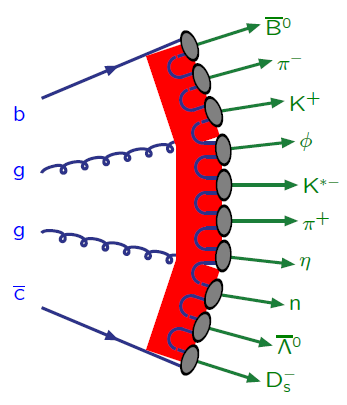
\includegraphics[width=0.6\textwidth]{figures/EvtGen/string.png}
  \captionsetup{width=0.85\textwidth} \caption{}
  \label{sec:evtgen:fig:cluster}
\end{subfigure}
\begin{subfigure}{0.5\textwidth}
  \centering
  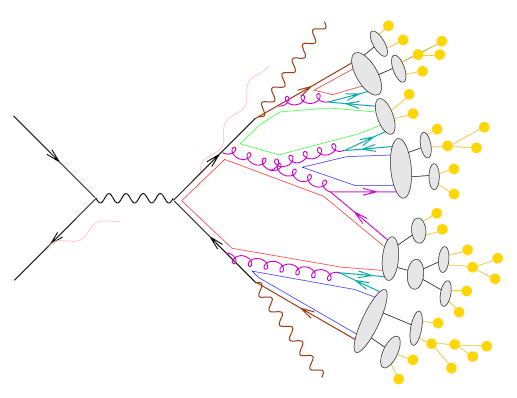
\includegraphics[width=0.9\textwidth]{figures/EvtGen/cluster.png}
  \captionsetup{width=0.85\textwidth} \caption{}
  \label{sec:evtgen:fig:string}
\end{subfigure}

\captionsetup{width=0.85\textwidth} \caption{\small The models of (a) string fragmentation and (b) cluster hadronisation.}
\label{sec:evtgen:fig:hadro}
\end{figure}

\subsection{Underlying event}

The processes discussed so far, i.e. the hard process, its higher-order corrections (parton shower) and development (hadronisation), are initiated by one parton from each incoming proton, neglecting  any effects of rescattering and the exchange of multiple partons between the initial-state protons. However, the event development receives a contribution from additional soft or moderately-hard processes, jointly referred to as ``underlying event'' (UE). The description of the UE employs phenomenological models, because of the non-perturbative nature of the processes involved. The  UE is considered to be composed of thee dominant components: multiparton interactions, beam remnants and pileup.\par
Multiparton interactions (MPI) correspond to moderately-hard interactions of the spectator partons among the incoming protons, i.e. those partons not participating in the hard process. The first detailed MC model for perturbative MPI was proposed in \cite{Sjostrand:1987su}. In this model, the crucial observation is that the t-channel propagators go on shell at low $p_{\bot}$, causing the differential cross sections to become very large. At the LHC  this parton-parton cross section becomes larger than the total hadron-hadron cross section at $p_{\bot}$ scales of order $4-5$ \gev (see figure \ref{sec:evtgen:fig:mpi}). In the context of MPI models, this is interpreted to mean that each hadron-hadron collision contains several few-$\gev$ parton-parton collisions. MPI interaction typically results in a pair of low-$\pt$ back-to-back jets that are colour connected with the rest of the event.

\bfig[h!]
\centering
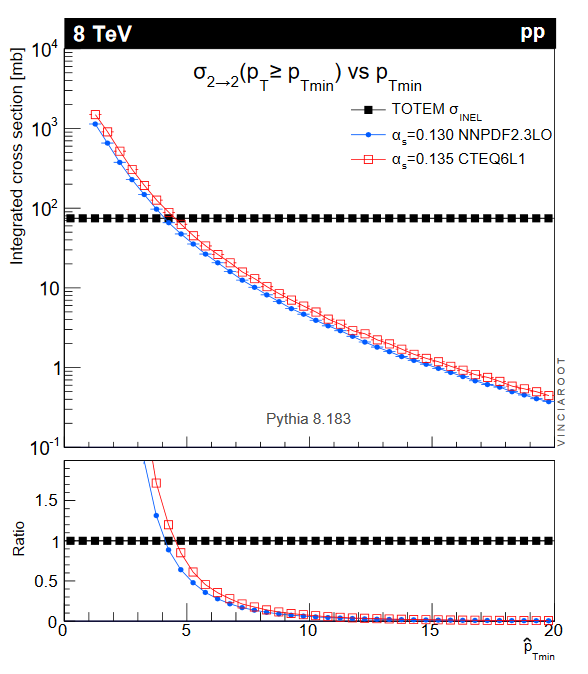
\includegraphics[width=0.5\textwidth]{figures/EvtGen/mpi.png}
\captionsetup{width=0.85\textwidth} \caption{\small Comparison of the total inelastic proton-proton cross section at $\sqrt{s}=8$ $\tev$ as measured by TOTEM, with the parton-parton cross section at LO in QCD as a function of the minimum parton $p_T$ ($\hat{p}_{{\rm T}{\rm min}}$). The fact that the curves cross at a scale of $\sim5$ $\gev$ is interpreted to mean that this is a characteristic scale relevant for MPI. From reference \cite{Skands:2012ts}.}
\label{sec:evtgen:fig:mpi}
\efig

Incoming beam particles may leave beam remnants that have not undergone any inelastic scattering. These remnants represent the soft QCD activity and need to be put together and colour connected with the rest of the event. What is left in the beam remnant is then a number of partons, with flavours given by the remaining valence content plus the number of sea quarks required for overall flavour conservation. Gluons in the remnant are not explicitly accounted for but are implicit as confinement clouds around the quarks.  Beam remnants are modelled by conserving the colour connection and momentum within the event.\par
Pileup, as discussed in section \ref{chp:det:LHC:design}, refers to the presence of additional inelastic $pp$ collisions in the event originating within the same bunch crossing (in-time) or from an event in a different bunch-crossing (out-of-time). Pileup represents a serious challenge to the reconstruction of the hard process as the products of pileup events largely overlap with those of the hard process (although in the case of in-time pileup typically originating from a vertex displaced with respect to that of the hard scattering). In-time pileup consist of soft QCD interactions and are modelled in a similar way as the UE. Out-of-time pileup is modeled with the same physics process, but considering interactions in past bunch crossings and simulating the time response of the readout electronics. In chapter \ref{chp:obj} several techniques to mitigate impact of pileup on reconstructed objects will be discussed.


\subsection{Event generators}

Event generators are tools that simulate collision events and their development, using the MC method. Generators can be either general-purpose, performing all steps in the event development, or specialised for a particular step of the event generation. Commonly used generators differ in the approach to various elements of event generation. While some use only a LO matrix-element calculation, others include higher-order corrections, as well as various parton-shower or hadronisation models. In this section, the general features of the generators used in the studies documented in this dissertation are briefly summarised.

\subsubsection{General-purpose Monte Carlo generators}

\bi
\ib {\sc Pythia} \cite{Sjostrand:2006za,Pythia8} is a MC generator using LO calculations for $2\to n$ $(n\leq3)$ processes, it can simulate collisions at high energies between elementary particles such as $e^{+}$, $e^{-}$, $p$ and $\bar{p}$ in various combinations. It contains theory and models for a number of physics aspects, including hard and soft interactions, parton distributions, initial- and final-state parton showers (emissions ordered in transverse momentum), multiparton interactions, fragmentation (Lund string model) and decay.
\ib {\sc Herwig} \cite{herwigpp} has the same capabilities as {\sc Pythia} with few small differences. It computes $2\to2$ processes using LO matrix elements. The parton-shower approach includes colour-coherence effects, with special emphasis on the correct description of radiation from heavy particles, and features emissions ordered in opening angle. The formation of hadrons from the quarks and gluons produced in the parton shower is described using the cluster hadronisation model. {\sc Herwig} is typically interfaced with the standalone software {\sc Jimmy} \cite{jimmy} that simulates the UE.
\ib {\sc Sherpa} \cite{Gleisberg:2008ta} is a multi-purpose MC generator that can provide multileg NLO/LO calculations (ME-PS matching uses CKKW method both at NLO and LO) It can simulate collisions between $e^{+}$, $e^{-}$, $p$ and $\bar{p}$ in various combinations. It contains theory and models for a number of physics aspects including BSM processes. It contains its own parton shower algorithm based on the Catani-Seymour dipole formalism \cite{Schumann:2007mg} and its own UE modelling. It can be interfaced with {\sc OpenLoops} \cite{Cascioli:2011va} to compute loop amplitudes and {\sc Comix} \cite{Gleisberg:2008fv} to generate matrix element amplitudes. 
\ei

\subsubsection{Matrix Element Monte Carlo generators}
\bi
\ib {\sc Powheg-Box} \cite{powheg} is an NLO parton-level generator using the {\sc Powheg} method  \cite{powbox1}. It generates the hardest radiation in the event using the exact NLO matrix element and is normally interfaced with another parton-shower MC generator (usually {\sc Pythia} or {\sc Herwig}) for showering, hadronisation and UE modelling.
\ib {\sc MadGraph5$\_$aMC@NLO} \cite{Alwall:2014hca} is an automated MC generator of LO/NLO matrix elements. The NLO calculation implements the {\sc MC@NLO} method \cite{mcatnlo_1}. It is normally interfaced with another parton-shower MC generator (usually {\sc Pythia} or {\sc Herwig}) for showering, hadronisation and UE modelling. It can perform ME-PS merging LO using the MLM prescription and at NLO using the FxFx method. It contains theory models and new ones can easily be added using UFO models \cite{Degrande:2011ua}.  
\ib {\sc Protos} \cite{protos}  is a LO ME generator for some BSM processes involving the top quark.  It can be  interfaced with {\sc Pythia} for showering and hadronisation.
\ei

\subsubsection{Specialised Monte Carlo generators}
\bi
\ib {\sc Photos} \cite{PhotosPaper} is a MC generator used to model bremsstrahlung in particles decay. It runs after parton shower ({\sc Pythia} or {\sc Herwig}) on the HepMC event record.
\ib {\sc Tauola} \cite{TauolaPaper}  is MC event generator that simulates tau decays for both leptonic and hadronic  decays  modes. It runs after parton shower ({\sc Pythia} or {\sc Herwig}) on the HepMC event record.
\ib {\sc EvtGen} \cite{Lange:2001uf} is  a MC that implements a detailed description of the physics of $b$-hadrons. In particular, it includes detailed models for semileptonic decays, CP-violating decays, and produces accurate results for angular distributions in sequential decays, including all correlations. It runs after parton shower ({\sc Pythia} or {\sc Herwig}).
\ei


